\startchapter{Related Work}
\label{chapter:problem}

\section{Misc Notes}

\cite{Bos98} mentions that Modula-3 is used as the first year language at the State University of New York at Stony Brook, and also has a rather lengthy discussion of why Java is a poor choice as first language.

``The MIT computer science department in 1997 replaced C++ with Java as the primary software language that students were required to learn'' \cite{Benander04}  It now looks like they are moving to Python.

MIT move from Scheme to Python: http://tech.mit.edu/V125/N65/coursevi.html

\cite{Benander04} has great numbers and figures on how various institutions have moved to Java.  Also provides very strong evidence to support the claim that Java is much easier to learn if you already know OO.  Also has support for the claim that Java is easy to learn if you are already experienced as a programmer, thus possibly lend more support to the notion of ``functional first'' (though be careful, it says Java is easy to learn if you know how to program, it doesn't say Java is easy to learn if you know FP).

\cite{Necaise08} indicates that the popularity of python is the removal of syntax issues -- possible motivation for VPE's?

\section{Practices of Teaching Introductory Programming}

\begin{flushright}
\textit{So, if I look into my foggy crystal ball at the future of computing science education, I overwhelmingly see the depressing picture of ``Business as usual''.}
\\
Edsger W. Dijkstra \cite{Dijkstra89} \\
\end{flushright}

In this section we explore how computer programming has been, currently is, and will be taught at various post-secondary institutions.  A thorough survey of literature surrounding how programming has been and is currently being taught can be found in \cite{Pears07}.

\subsection{Curricula}

\begin{flushright}
\textit{We're not a vocational school. If someone wants to get a high-paying job, I would hope that there are easier ways to do it than working through a formal computer science curriculum.}
\\
Philip Greenspun \cite{Greenspun00} \\
\end{flushright}

Introductory programming courses should always be considered within the context of the curriculum in which they lie.  Traditionally, the introductory programming course was one of the first (or was the first) course students undertaking a degree in Computer Science would enroll, as many future Computer Science courses assume basic programming experience as a basic skill.

In North America, many introductory computing courses follow the guidelines outlined in the Computing Curricula recommendations by the ACM and IEEE Computer Society Joint Task Force.  The latest full curriculum recommendation came in 2001 (known as CC2001)\cite{cc2001}.  In 2008 an interim revision from the task force was submitted\cite{cs2008}.  CC2001 identified 14 areas which comprised the body of knowledge for computer science at the undergraduate level.  These are listed in \tref{tab:CC2001BOK}.

\begin{table}
	\caption{The 14 Areas Which Comprise the CC2001 Body Of Knowledge For Computer Science}
\begin{tabular}{l}
Discrete Structures (DS) \\
Programming Fundamentals (PF) \\
Algorithms and Complexity (AL) \\
Architecture and Organization (AR) \\
Operating Systems (OS) \\
Net-Centric Computing (NC) \\
Programming Languages (PL) \\
Human-Computer Interaction (HC) \\
Graphics and Visual Computing (GV) \\
Intelligent Systems (IS) \\
Information Management (IM) \\
Social and Professional Issues (SP) \\
Software Engineering (SE) \\
Computational Science and Numerical Methods (CN) \\
\end{tabular}
	\label{tab:CC2001BOK}
\end{table}

Each of these areas are subdivided into units, and each unit consists of a number of topics.  Of the various units, some are given additional \emph{weight} in the recommendation by being designated as \emph{core} units, which are intended as being fundamental to \textbf{any} student of computer science irregardless of area of emphasis.  All units which are not designated as core units are referred to as \emph{elective} units.  While the core units comprise a fundamental set of topics for computer scientists, by themselves the core units (and the topics within) do not comprise a \emph{complete} set of material for a computer scientist -- they need to be supplemented with other elective units from other areas depending on the area of emphasis, the needs and goals of the education institution, etc.

For many years, this task force proposed a two-course introductory programming sequence commonly generically referred to as the CS1/CS2 sequence.  Most educational institutions in North America have followed this pattern, though the contents of the courses have evolved over time.  Roughly speaking, traditionally CS1 tends to focus on introductory programming concepts (control flow and conditional statements, variables, iteration, etc), and CS2 tends to focus more on the introduction of data structures (trees, queues, etc).  In CC2001, the importance of the object-orientated paradigm was recognized, and it was suggested that object-orientated concepts become a central part of the introductory course sequence.  Partly as a result of this addition, CC2001 also suggested a third course to follow CS2 (typically called CS3) to ensure ``students are able to master these fundamental concepts before moving on''\cite{cc2001}.  Adoption of the three course model has been mixed, with many institutions retaining the two course sequence.

\subsection{Pedagogy}

\begin{flushright}
\textit{If I could have one wish for education, it would be the systematic ordering of our basic knowledge in such a way that what is known and true can be acted on, while what is superstition, fad, and myth can be recognized as such and used only when there is nothing else to support us in our frustration and despair.}
\\
Benjamin S. Bloom \cite{Bloom72} \\
\end{flushright}

Whereas the curriculum outlines the topics that shall be introduced in a computer science curricula, an equally important (perhaps more important) aspect of the teaching of how to program is that of pedagogy.  The difference between curricula and pedagogy is well described by Pears, et al, as ``While the curriculum defines what is to be taught, pedagogy deals with the manner in which teaching and learning are managed in order to facilitate desired learning outcomes''\cite{Pears07}.  More roughly speaking, the curriculum is the ``what'' and pedagogy is the ``how''.

In the relatively short history of the discipline, there have been a number of approaches to how to introduce students to the world of computer programming.  One of the most hotly debated issues is that of the paradigm to use early on.  Traditionally, the Computing Curricula recommendations by the ACM and IEEE Computer Society Joint Task Force suggested a ``programming-first''\footnote{Sometimes this approach is referred to as ``procedural-first'', sometimes ``imperative-first''.} approach.  This style emphasized a procedural programming style early on, and many institutions still follow this model today.  However, it has been argued that this approach furthers the misconception that ``computer science equals programming'', as it puts such a heavy emphasis on programming perhaps at the expense of topics (particularly theoretical topics) more central to the discipline \cite{cc2001}.  Additionally, it has also been argued that a programming-first approach unfairly favours students with prior programming backgrounds over students with little or no background.  In addition, students who have learned some programming skills on their own before the introductory programming class tend to not have the opportunity to have poor habits corrected in the programming-first approach, as the emphasis of the approach is on simple syntactic details rather than design and algorithmic problem solving \cite{cc2001}.

As a result of many of these criticisms and potential shortcomings, as well as the increased prevalence of the paradigm, CC2001 suggested the incorporation of object-orientated principles into their introductory programming sequence.  This ``objects-first'' approach has been the source of much debate in academia since 2001 when the suggestion was made in the CC2001 guidelines, and in particular during a well documented e-mail discussion on the SIGCSE mailing list in 2004 \cite{Pausch03,Astrachan05,Hu04,Lister06}.  Some feel that the subtleties, complexities, and level of abstraction required of the object-orientated paradigm represent too great an intellectual leap for introductory programming students\cite{Hu04,Lister06}.  Some believe that the CS1/CS2 curricula is already ``too full'' as it is, without the additional complexities of the OO paradigm, and that introducing OO into the CS1/CS2 sequence will cause traditional programming constructs to be pushed to the wayside\cite{Hu04}.  Some argue that the OO paradigm is an extension of the procedural, and thus procedural programming needs to be fully understood before objects can be discussed\cite{Lister06}.  Some of the reasons for introducing objects early include the belief that since the OO paradigm is the most dominant in the world of computing, and will continue to be so for the foreseeable future, many believe that as such it is the most important for students to learn, and thus should be the first that they learn\cite{Pausch03}.  Additionally, another one of the common difficulties associated with learning the OO paradigm is that of ``paradigm shift'', and as such it has been argued that if we begin with objects early, then we avoid the paradigm shift problem\cite{Hu04,Lister06}.

In parallel to the programming-first to objects-first evolutionary approach to pedagogy, some have argued for the incorporation of functional programming into early programming courses, and propose a ``functional-first'' approach.  Much of the roots of this approach come from the text ``Structure and Interpretation of Computer Programs''\cite{SICPbook}, which was a highly influential text during the 1980's\cite{Flatt04}.  SICP, as it is commonly referred, made use of the functional programming language Scheme, and many of the exercises in the text discussed and relied on concepts from the functional paradigm (the lambda calculus, higher order functions, etc).  A well-known criticism of SICP was written by Wadler in 1987 which criticized the use of Scheme as the language, but argued in favour of retaining the functional focus of the text\cite{Wadler87}.  There has also been research done which would indicate that perhaps beginning in the object-orientated paradigm is a less desirable choice than beginning in the functional paradigm\cite{Flatt04,Huch05}.  This has significant repercussions in terms of language choice, as (for example) Java is a heavily object-orientated language, and as such it has been argued is not the ideal choice for a first year course\cite{Bos98,Huch05}.  The TeachScheme/ReachJava project shows that ``functional first'' does not imply that object-orientation must be avoided in the first year of study \cite{Bloch08,teachScheme,Felleisen04}.  Concerns with ``functional first'' include the notion that sometimes concepts that are more difficult to express in the functional paradigm are sometimes given diminished importance (I/O being the most prominent example), concerns about introducing recursion early, and the notion that functional programming is not ``mainstream'' (thus raising the ``this isn't really used out in the real world'' criticism)\cite{Chakravarty04}.

In any case, all of these approaches (programming-first, objects-first, and functional-first) share a common characteristic -- they are all based upon the notion that we should structure our approach to teaching introductory programming around a particular programming paradigm.  Some however feel that this is inappropriate, that rather than focusing on a particular programming style, we should be focused on more general concepts and ideas irregardless of the paradigm.   Most notably, there has been a move toward a ``design-first'' instructional style for the introductory course.  Traditionally introductory programming courses are taught by example.  The instructor introduces a new syntactic construct from the language being used, shows a number of examples using this construct, then exercises or assignments are given where students have to take the given code from the instructor and modify it to a new problem.  Some people feel that this approach emphasizes the language more than design, and given that the specific language in use is not the primary goal of the course, it has been argued that this creates courses whereby students walk away feeling as though programming is all about learning syntax, and not about designing creative solutions to interesting problems.  The consequence of this approach is that it makes the teaching of syntax explicit and the teaching of design implicit, potentially causing courses to create students who can take existing code in Java or C++ (whichever language is used) and modify it to a new problem, but cannot design a solution to a problem from scratch.  \cite{Flatt04} outlines a course whereby design is made much more explicit to students, and has reported success in their approach.  What is interesting about this approach and others which claim to put general issues such as design as the focus, is that they are almost exclusively rooted in the functional paradigm.

\subsection{Language Choice}

\begin{flushright}
\textit{The limits of my language mean the limits of my world.}
\\
Ludwig Wittgenstein \cite{Wittgenstein22} \\
\end{flushright}

The choice of programming language is a critical one, though perhaps an overstated one.  Ideally the introductory programming course should be a course which teaches systematic thinking and problem solving, not ``how to write Java''.  Thus, while by necessity the introductory programming courses must make use of a programming language and environment, the primary goal of the introductory course is to teach programming in the abstract sense rather than specific syntax.

\begin{comment}
FIXME maybe drop this para:
In the history of the field, computer science has seen a variety of languages employed at one time or another as being ``the teaching language of choice''.  For our purposes we shall outline three time-frames and list some of the languages most commonly in use during those times as well as summarize findings in regards to the successes and failures of those languages from a pedagogical standpoint.
\end{comment}

In the history of the field, computer science has seen a variety of languages employed at one time or another as being ``the teaching language of choice''.  Almost as varied as the number of languages employed is the number of reasons why one language has been chosen over another.  Sometimes a language is chosen based upon faculty preference, sometimes because of industry prevalence.  Some languages are designed with learning in mind and as such have a certain appeal to educators.  Sometimes support materials in the form of programming environments or documentation will sway a department from using one language to using another.  Sometimes the paradigm chosen plays a prominent role\footnote{It would seem odd to try and teach object orientated programming in Haskell for example, as that language is based upon a different paradigm}.

Today C, C++, and Java are the most commonly used languages in both industry and education\cite{Pears07}.  Part of the appeal of these languages include the fact that they tend to be the ones most heavily used in industry.  There is additionally a sense of a movement away from C and C++ to Java as time is progressing\cite{Benander04,Bruce05}.  Various reasons have been proposed for this movement, the most common seems to be that it is a reflection of the increasing adoption of Java in industry\cite{Benander04}.  There has been considerable work done in collecting and producing resources to aid educators who are using Java in their first year courses.  One of the most prominent is the ACM Java Task Force\cite{Roberts05}.

There has been considerable debate however as to whether or not Java is the most appropriate choice of language for introductory programming courses\cite{Bruce05}.  It has been shown that certain background characteristics are highly correlated with success in learning introductory programming courses for which Java is the language of choice.  The most prominent of these characteristics is prior familiarity with the object-orientated paradigm\cite{Benander04}.  This is not entirely surprising given how the language is heavily based upon that paradigm, however it is troublesome from an educational point of view in that one of the reasons Java is used in introductory programming courses is that because it is an object orientated language it has been argued that it is a suitable choice for an ``objects-first'' approach.  Furthermore, it has been recognized that most of the programming tools which have been adopted are primarily aimed at the Java programming language.  What is not clear is whether or not this is due to a relatively widespread acceptance of the Java language, or if it is a reflection of the need for additional learning support with that language\cite{Pears07}.

Additionally there are language-specific concerns that have been raised with Java.  The ACM Java Task Force identified a Taxonomy of Problems in Teaching Java\cite{acmJavaForce04}, some of which have been somewhat addressed as the language has evolved, and some of which remain problems to this day.  The difficulties are summarized in \tref{tab:ACMJTFPROB}.

\begin{table}
	\caption{Summary of Problems in Teaching Java\cite{acmJavaForce04}}
\begin{tabular}{c p{3in} r}
\hline
\multicolumn{3}{l}{\emph{High Level Issues}} \\
H1 & Scale & (remains a concern) \\
H2 & Instability & (remains a concern) \\
H3 & Speed of Execution & (improving over time) \\
H4 & Lack of good textbooks and environments & (improving over time) \\
\hline
\multicolumn{3}{l}{\emph{Language Issues}} \\
L1 & Static methods, including \code{main} & (remains a concern) \\
L2 & Exceptions & (remains a concern) \\
L3 & Poor separation of interface and implementation & (partly addressed by tools) \\
L4 & Wrapper classes & (added in Java 5.0) \\
L5 & Lack of parameterized types & (added in Java 5.0) \\
L6 & Lack of enumerated types & (added in Java 5.0) \\
L7 & Inability to code preconditions & (added in JDK 1.4) \\
L8 & Lack of an iterator syntax & (added in Java 5.0) \\
L9 & Low-level concerns & (disposition varies) \\
\hline
\multicolumn{3}{l}{\emph{API Issues}} \\
A1 & Lack of a simple input mechanism & (remains a concern) \\
A2 & Conceptual difficulty of the graphics model & (remains a concern) \\
A3 & GUI Components inappropriate for beginners & (remains a concern) \\
A4 & Inadequate support for event-driven code & (remains a concern) \\
\hline
\end{tabular}
	\label{tab:ACMJTFPROB}
\end{table}

As the result of the difficulties associated with the use of C/C++ and Java in the introductory programming course, many institutions are now switching from C/C++ and/or Java to other languages.  The most common of these being the Python programming language \cite{python}.  Python has the advantage of being a scripted, interpreted language, thus students can ``try-out'' small expressions or snippets of code without having to get a complete source file free from errors.  It also has a relatively ``clean'' and simple syntax compared to the relatively verbose Java.  The use of whitespace for program structure encourages good indentation habits early as well.  With all these benefits it is not surprising to see some institutions beginning to adopt Python as the language for their introductory programming courses.  Perhaps the most notable adoption of Python happened at MIT, whose Computer Science department had long been a strong proponent of the use of Scheme in introductory programming courses due to the adoption of \cite{SICPbook} as the introductory text \cite{Thetech06}.  Other examples of using Python in CS1/CS2 style courses and the possible benefits and drawbacks of doing so can be found in \cite{Radenski06,Shannon03,Agarwal05,Agarwal08}.  While there have been successes with Python in the classroom, not even the strongest supporters of the language claim that it is the ``perfect choice''.

\section{Visual Programming Environments}
\label{sec:vpes}

One of the major difficulties associated with learning to program is the issue of syntax errors\cite{Kelleher05}, and as a result of this, there has been a great deal of work done attempting to minimize or reduce this hurdle.  One of the major categories of this work is the world of the visual programming environment (VPE)\footnote{Some authors use the term ``visual programming language'' rather than ``visual programming environment''}.  A VPE is a programming environment where the user interacts with graphical on-screen objects rather than the traditional textual method of writing text-based code.  Another definition comes from Kelleher \& Pausch:

\begin{quotation}
...[VPE's] use graphical or physical objects to represent elements of a program such as commands, control structures, or variables. These objects can be moved around and combined in different ways to form programs. Novice programmers need only to recognize the names of commands and the syntax of the statements is encoded in the shapes of the objects, preventing them from creating syntactically incorrect statements\cite{Kelleher05}.
\end{quotation}

\subsection{Criticisms of Visual Programming Environments}

There are two common criticisms of VPE's that have somewhat slowed their adoption: the scaling-up problem, and concerns about transfer of training.  The scaling-up problem refers to the programmer's ability to apply VPE's in larger programs.  That is, questions have been raised about whether or not the visual representation used in VPE's ultimately are too unwieldy to produce programs of moderate complexity\cite{Burnett94}.  Transfer of training concerns whether or not skills and knowledge acquired in a VPE can be transferred to a traditional text-based environment in the future.  Some support for the claim that a visual environment can provide positive ``transfer of training'' to a textual environment can be found in \cite{Hundhausen09}.

\subsection{Examples of Visual Programming Environments}

There have been a number of VPE's proposed, we shall focus on a few environments which have proven to be of great influence particularly in regards to the educational side of Computer Science.  A more thorough discussion of other VPE's can be found in \cite{Kelso02} and \cite{Kelleher05}.

An early VPE system that has proven to be quite influential is Prograph, a visual object-orientated dataflow language.  Objects in Prograph are modeled as on-screen hexagons, with one half of the hexagon representing the data attributes of the object, and the other half the methods.  By double-clicking on a part of the object a user can explore further the various methods and attributes of the object.  Methods are contained in ``frames'', which are represented as directed graphs.  Nodes in the graph are icons representing various constructs (objects, methods, conditionals, etc) and are connected together.  Flow of data proceeds from the top of the digraph, passing through the various instructions, down to the bottom of the digraph, and outward (if the method has output).  One of the major influences of Prograph was this ``box and wire'' representation, as it was one of the earlier systems to make use of it, and many VPE's have also made use of this metaphor.  As well, Prograph has become something of a benchmark system in evaluating VPE's\footnote{Green uses Prograph and Labview as the two model systems which he applies his Cognitive Dimensions Framework to}.  It would appear however, that active development on Prograph ceased in the early 1990's.

Another VPE that is somewhat similar to Prograph is Labview\cite{labview}, a visual environment used for designing electronic circuits.  That is, it uses ``the metaphor of an electric circuit as a programming model''\cite{Kelso02}.  It also has a dataflow-style, whereby components are connected together, and data ``flows'' through the network of components.  It also, like Prograph, makes use of the ``box-and-wire'' representation.  It is a proprietary product of the National Instruments corporation, and also has been used as a ``model'' language when evaluating VPE's.

Neither of the above two environments are based upon the functional paradigm however.  One such environment that is heavily based upon the functional paradigm is the VFPE\footnote{Short for ``Visual Functional Programming Environment''}, developed by Kelso \cite{Kelso02}.  The VFPE shares a common computational model with existing functional languages (such as Haskell).  One of the central points of Kelso's work is the argument that functional languages have a unique singular visual representation -- the syntax tree.  As such, the VFPE is in many ways just a visual representation of that tree.  A screenshot of the VFPE can be seen in \fref{fig:vfpe}.  The main interface to the VFPE consists of a main expression window (seen in \fref{fig:vfpe-main}) which contains the program being constructed.  Components are selected from the menus on the right half of this interface, and dropped into placeholders in the main expression.  Functions can be defined, and the definition of sub functions are done in a separate window called a binding frame (as seen in \fref{fig:vfpe-sub}).  Note that the layout of components is done by the environment, it is not ``freeform'' as users cannot control where components are laid out in the main expression window.

\begin{figure}[htp]
  \begin{center}
    \subfloat[The Main VFPE Window]{\label{fig:vfpe-main}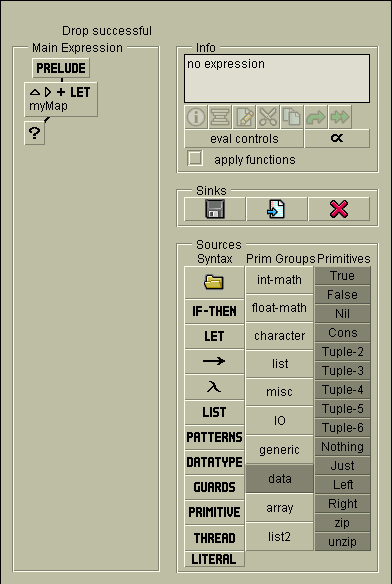
\includegraphics[scale=0.4]{Figures/vfpeMain}} \quad
    \subfloat[A Binding Frame in VFPE]{\label{fig:vfpe-sub}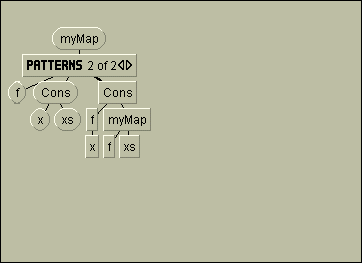
\includegraphics[scale=0.4]{Figures/vfpeSub}}
  \end{center}
  \caption{The Visual Functional Programming Environment (VFPE)}
  \label{fig:vfpe}
\end{figure}


Alice, Scratch, Gamemaker, VFPE, Prograph


Use of Game Maker in educational setting at UVic can be found in \cite{Gooch08}.


\section{Games and Computer Science Curricula}
\label{chapter:problemSec:games}

In recent years there has been a notable decline in enrollment in Computer Science courses \cite{Manaris07,Vesgo07,Ward08,Bayliss09}.  As a result of this decline, many institutions are seeking out interesting and new ways to ``entice'' students to enroll in Computer Science courses and to rekindle interest in the discipline.  One such method that has been proposed is to incorporate computer games into Computer Science curricula.  Cliburn et al. provides a summary of how games have been used in this fashion in \cite{Cliburn06}.

The rationale behind this move is that since video games are an exciting and compelling application of computer programming, that perhaps that interest in games can be leveraged by instructors in their introductory programming courses and beyond \cite{Barnes08,Sweedyk05,Overmars04}.  Furthermore, video games are a multi-billion dollar industry \cite{Wallace06}, and a common motivation for students in choosing a discipline are the employment opportunities a degree in the field would entail.  Since electronic entertainment is so prosperous, having curricula that targets students specifically for this field can be a compelling factor in one choosing a degree in Computer Science.

Some institutions have even taken this move a step further and are now offering gaming themes and concentrations in their degrees.  Recently, the University of Victoria added a ``Graphics and Gaming'' option to their Computer Science major program.  Other attempts at this are explored in \cite{Leutenegger07,Murray06,Zyda06}.  Most institutions that incorporate games into their courses or degrees have reported an increase in student enjoyment.  It has been shown that students prefer assignments based around games than ``traditional'' or ``story-telling'' assignments \cite{Cliburn08}.

%\cite{Cliburn08} provides strong evidence that in a general, aggregate study, students prefer assignments based around games than ``traditional'' or ``story-telling'' assignments.

While there have been successes reported surrounding the use of games, it is very much a controversial choice, as there are a number of concerns that have been raised in regards to gaming-centered curricula.  There is strong evidence to indicate that while gaming may spark initial interest in computing, it does not follow that this initial interest will translate into increases in students undertaking Computer Science majors.  A survey of 1,872 students conducted at a ``highly selective public technical university'' found that while 43\% of students indicated that games influenced their interest in computing, only 6.9\% realized that interest by becoming Computer Scientists \cite{DiSalvo09}.  Furthermore, while student interest generally seems to increase with assignments making use of games, few institutions have reported any noticible improvement in student performance.  Cliburn reported findings of a study he performed in the introductory programming course at Hanover College and found that students had a higher overall average score (95.1\% on average) on traditional assignments than on game-based assignments (89.1\% on average)\cite{Cliburn06}.  Interestingly, he also found that in spite of this, most students (78.9\%) still preferred game-based assignments over ``traditional'' assignments, perhaps a further testament to the motivating power of games as assignments.

Concerns have also been raised surrounding issues of gender and race.  One such concern suggests that games appeal more to male students than female, and that incorporation of games may alienate females from the discipline.  Specifically, there has been evidence to show that females tend to prefer games which are cooperative in nature rather than competitive, and that the latter can deter interest of women in games \cite{Camp02}.  This would indicate that educators must be careful about how they incorporate games into courses, and to design course materials with this concern in mind \cite{Carmichael08}.  Other works have adopted ``story-telling'' rather than games as being the vehicle of motivation, and have specifically explored this avenue with middle-school girls with great success \cite{Kelleher06}.

\begin{comment}
\cite{Natvig04,Barnes08} example of games being used
Some ideas about why creativity is important can be found in \cite{Farooq06}.
Games as a motivational tool: see ``International Conference on Game Development in Computer Science Education''.
An excellent outline of how games can be used successfully in CS curricula as well as how not only should we shoehorn games but also focus on fundamentals is summarized in \cite{Bayliss09}.  It also discusses what considerations should be made when incorporating games into courses.
\end{comment}

\section{The Cognitive Dimensions Framework}
\label{chapter:problemSec:cgframework}

One of the challenges faced in evaluating a programming environment is that programming is such a \textit{subjective}
task.  Different programmers have different preferences, and value certain features over others.  While one
programmer may find one aspect of the environment very useful, another may find that aspect counterintuitive.  
Programmers are famous for being extremely opinionated about the tools and environments they use, developing almost
dogmatic devotion to one approach at the expense of others.  It can be difficult to find a formal method to
use to discuss the merits of one language design over another that can be agreed upon.

When computer scientists and software engineers try to evaluate the usability of a system, they turn
to human computer interaction (HCI) principles to do so.  However, as pointed out in \cite{green96}, this is 
problematic for the evaluation of programming environments as typically HCI tends to focus on interactive situations
rather than notational design.  That is, HCI tends to focus more on ``micro-tasks'' and the finished product, rather
than the processes and activities which produce that task.  As an example, in evaluating a programming environment it is less important
to know that the ``compile'' option is easy to find than it is to know that the environment does not allow for new 
abstractions to be created.  Moreover, programmers are not HCI experts, and
vice-versa.  Thus while the vocabulary of HCI may be second nature to those in the field, it is less so for the
average computer programmer or software engineer.  Similarly, it is not uncommon for programmers to use terminology
that is unfamiliar to those who are not software developers.  For our purposes, we shall use the ``cognitive dimensions 
framework'' outlined by Green in \cite{green96} for evaluating differing visual programming environments.  

In this section we will outline the cognitive dimensions framework, giving an overview of the various dimensions of the framework, as well as recap some of the ways in which it has been applied to other environments.

\subsection{Outline of the Cognitive Dimensions Framework}
\label{cgframeoutline}

The Cognitive Dimensions Framework consists of 13 different ``dimensions'' to easily evaluate and critically examine a programming
environment.  The purpose of the framework is to provide a set of 
dimensions which capture much of the psychology and HCI of programming, and give a vocabulary for which VPL
designers and users can use to examine different visual programming environments.  It is less of a framework
for stating that ``language X is better than language Y'', but more for statements like ``language X can have
better Y by changing Z'' (where Y is one dimension of the framework, and Z is some aspect of the VPE that
impacts Y).  Furthermore, the language used in the framework is more accessible to the average software developer, 
not requiring one to be an HCI expert to use it.

One very important aspect of the framework is that (not surprisingly) different dimensions can represent trade-offs.  In fact, 
this is intentional --- there are always trade-offs in designing any system of moderate complexity, and until there is a 
vocabulary for discussing those trade-offs it is difficult to reason about how one can improve the initial design.  The cognitive 
dimensions framework is intended as being able to fill this void, allowing designers to coherently and critically examine 
and \textit{converse} about their designs so that they may find the best compromise given the objective(s) of the system 
being designed.  As Green himself puts it ``Like other forms of engineering, design is a matter of compromise''. \cite{green96}

Below is a recap of the listing of the thirteen dimensions of the Cognitive Dimensions Framework described by Green in \cite{green96}. 

\begin{itemize}
	\item Abstraction Gradient - What are the minimum and maximum levels of abstraction?
	\item Closeness of Mapping - What programming ``games''	need to be learned?
	\item Consistency - When some of the language has been learned, how much of the remaining parts of the language can be inferred?
	\item Diffuseness - How many symbols or graphic entities are required to express a meaning?
	\item Error-proneness - Does the design of the notation induce ``careless mistakes''?
	\item Hard Mental Operations - Are there places where the user needs to resort to fingers or penciled annotation to keep track of what's happening?
	\item Hidden Dependencies - Is every dependency overtly indicated in both directions? Is the indication perceptual or only symbolic?
	\item Premature Commitment - Do programmers have to make decisions before they have the information they need?
	\item Progressive Evaluation - Can a partially-complete program be executed to obtain feedback on ``How am I doing?''
	\item Role-expressiveness - Can the reader see how each component of a program relates to the whole?
	\item Secondary notation - Can programmers use layout, colour, or other cues to convey extra meaning, above and beyond the `official' semantics of the language?
	\item Viscosity - How much effort is required to perform a single change?
	\item Visibility - Is every part of the code simultaneously visible (assuming a large enough display), or is it possible to juxtapose any two parts side-by-side at will?
\end{itemize}

A more detailed description of each is given in the sections that follow.

\subsubsection{Abstraction Gradient}
\label{absgradientoutline}

\cite{green96} describes the Abstraction Gradient as ``What are the minimum and maximum levels of abstraction?  Can 
fragments be encapsulated?''  Furthermore, Green classifies languages based upon three categories: abstraction-hating, 
abstraction-tolerant, or abstraction-hungry depending upon the languages minimum starting level of abstraction and their 
readiness or desire to accept further abstraction.

That is, this dimension asks the questions: how much needs to be constructed and learned in order to begin making the programming
environment perform a task?  And how easy is it to add new abstractions?  

The example Green gives of an abstraction-hating formalism is that of flowcharts, as they only allow decision boxes 
and action boxes.  There is no way to ``add'' additional constructs or group related ideas within a flowchart.  While they 
have a low minimum level of abstraction (there is not much to learn to begin using them), they have no readiness to accept
further abstractions.  Turing 
machines would be another example of a notation which is abstraction hating --- each instruction can only have a current 
state, current symbol, next state, next symbol, and a direction to move on the tape.

The classic example of an abstraction-tolerant language would be C, as it has a higher minimum level of abstraction (one must
learn some of the various keywords in the language, as well as how to write a \code{main()} routine for example), and it allows
for new abstractions of various kinds to be created (for example, one can create new types with \code{typedef} and \code{struct}).

The example Green gives of an abstraction-hungry language is Smalltalk, as it has a high starting level of abstraction, 
and requires one to modify the class hierarchy in order to create new programs.  That is, every program written in the
language \textbf{requires} the introduction of new abstractions.

From the perspective of learning to program, it has been shown that oftentimes
students new to computer programming struggle with languages which force one to learn and master several 
abstractions at once, giving them ``a `rubber hamburger' which has to be swallowed because it cannot be chewed''\cite{green96}.
As such it is difficult to find the right balance here, requiring too many abstractions to be learned can negatively
impact learning, but having limited abstraction mechanisms can make programs difficult to modify (see the section on Viscosity
later).  Green seems to indicate that abstraction-tolerant languages are the best fit for learning environments, but admits
that more research needs to be done in this area.

\subsubsection{Closeness of Mapping}
\label{closenessoutline}

One could argue that programming is all about problem solving.  Put another way, given a problem expressed in one particular domain (the problem domain) the role of the programmer is to come up with a mapping of this problem into the domain of the programming environment in use (the program domain).  Closeness of mapping tries to measure the gap between the problem domain and the program domain.  That is, how much extra ``administrative stuff'' does the environment impose upon the programmer in order to translate a solution to a problem into something that can be executed in the programming environment?  Green refers to this ``administrative stuff'' as ``programming games'', or the little language/environment-specific idiosyncrasies that are imposed upon the programmer.  The classic example of a programming game which is imposed on many first year computer science students is the \code{public static void main (String [] args)} method signature that must appear in any Java program.  This line is (typically) completely absent from the problem domain, yet is a required artifact that students must produce in order to produce a solution to any problem given to them by their instructors when Java is the language of choice.

Closeness of Mapping also is to a lesser degree a measure of what the environment provides in terms of standard libraries and constructs.  If a language provides a great deal of standard libraries, then intuitively it would seem that there would be less work for the programmer to do to create the mapping from problem domain to program domain.  Related to this is the notion of whether or not the language allows constructs to be built that improve the Closeness of Mapping.  That is, if functionality is not provided in the way of standard libraries, is it possible for one to add their own to better bridge the gap between
problem and program domain.

Traditionally (and not surprisingly), domain-specific languages tend to score very well in this regard \emph{when the problem lies within the target domain that the language was designed for}.  It is less clear as to how well these languages score when attempting general problems that fall outside of that targeted domain.

\subsubsection{Consistency}
\label{consistencyoutline}

Consistency tries to measure how easy it is to infer the remaining parts of the language once one has learned part of the language.  Put another way, consistency assesses whether or not ``similar semantics are expressed in similar syntactic forms''.\cite{green98}  Green states consistency as a form of ``guessability'': ``when a person knows some of the language structure, how much of the rest can be successfully guessed?''\cite{green96}  An example that has been given for a way in which a language suffers from consistency problems is Pascal and its handling of reals and integers versus boolean variables.  In Pascal, one can read and write to reals and integers, but boolean variables may only be read from even though syntactically booleans are essentially used and treated in the same way as other variables.

Another more modern example would be Java and its String data type.  Strictly speaking, \code{String}s are object types in Java, but can be treated in much the same way as primitive data types (such as \code{int}s or \code{boolean}s).  For example, one can use the concatenation operator to combine two strings together in infix notation as seen in \pref{prog:javainfix}.  This is the only time in which object types may be used in this ``operator overloaded'' way, all other object types must resort to method calls (as seen in \pref{prog:javamethod}).  ``Special cases'' such as this can greatly hurt the consistency of a language and make them harder to learn.

\begin{program}
\begin{verbatim}
String s1 = "Hello";
String s2 = " World";
String s3 = s1 + s2;  // create "Hello World" 
\end{verbatim}
\caption{Concatenating Two Java Strings Using an Operator in Infix Notation}
\label{prog:javainfix}
\end{program}

\begin{program}
\begin{verbatim}
String s1 = "Hello";
String s2 = " World";
String s3 = s1.concat (s2); // create "Hello World" 
\end{verbatim}
\caption{Concatenating Two Java Strings Using Method Calls}
\label{prog:javamethod}
\end{program}

Typically visual languages tend to score well in consistency, largely due to a simpler syntax.  Many textual-based languages have struggled in regards to consistency as most ``real-world'' textual languages have grammars of substantial size, and generally speaking the larger the grammar, the more complex the syntax (and thus the more likely there will be inconsistencies that arise).
 
Additionally, as noted by \cite{Kelso02} an issue related to consistency is that of library regularity.  For example, Haskell generally keeps naming and argument ordering in libraries in regular order (thus scoring well in terms of consistency).  C libraries however tend to not score so well, largely due to the fact that they have been developed over a long period of time by a large number of authors\footnote{As well, it could be argued that the fact that all functions in C reside in the same namespace negatively impacts consistency as well as it means that library designers must come up with their own unique naming schemes for functions to avoid naming conflicts.}.

It has also been noted that consistency can be viewed from two different perspectives: the learner and the designer. \cite{Reisner93} Ideally these two perspectives should be the same, but in practice they often are not.  The distinction in Java between object types and primitive types is an example of this.  From the designers perspective this is perfectly consistent -- there are two fundamental categories of data types, and within the Java Virtual Machine (JVM) they are handled completely differently and separately.  From a learner's perspective however, this distinction can create confusion.  From a learner (or user of the language) it is all just data so the distinction is not as apparent and, for many new to the language, seems rather arbitrary.

At any rate, given that the Cognitive Dimensions framework was designed by Green to be used by designers of a language one might think that his intention was that consistency was to be applied from the designers perspective, however this is not explicitly stated.  From our perspective as evaluators of a VPE from a pedagogical standpoint we are however more interested in the learners perspective, and our application of this dimension in evaluating the Gem Cutter will reflect this.

\subsubsection{Diffuseness}
\label{diffusenessoutline}

Diffuseness is also sometimes referred to as terseness.  That is, it tries to measure how many symbols (or graphic entities in the case of a VPE) are required to express a meaning.  This is, of course, a trade off -- if a language is too terse it can be hard to read, but if a language is too verbose it becomes difficult to ``keep it all in your head'' at once.

Traditionally functional languages have been quite terse, and scored well in that regard\footnote{Some even criticize functional languages for being \emph{too} terse, further illustrating that this dimension represents a trade-off.}.  Visual languages also tend to require a small number of syntactic elements to express a meaning, so one would think that a visual functional programming environment would be the most terse of all environments, and Kelso found this to be true of his VFPE\cite{Kelso02}.

Measuring diffuseness/terseness is done by counting the number of syntactic lexemes that comprise a program.  To give a meaningful comparison, Green uses a sample yardstick problem taken from \cite{curtis89} that he calls the ``rocket trajectory problem'' which he summarizes as:

\begin{quotation}
The rocket program computes the vertical and horizontal trajectory of a rocket on which the only forces acting are its thrust and gravity.  At time zero the rocket stands stationary and vertical on level ground, with a mass of $10^4$ pounds.  Its engine develops a thrust of $4\cdot10^5$ foot-pounds, using up a mass of 50 pounds of fuel per second, until the fuel is exhausted after 100 seconds.  It rises vertically for 10 seconds after which it adopts and retains an angle of 0.3941 radians (22.5 degrees) to the vertical.  The downwards acceleration of gravity is $32 feet/sec^2$.\cite{green96}\label{rocketproblem}
\end{quotation}

%in \fref{fig:rocketTrajectoryProblem}.  
%\begin{figure}
%The rocket program computes the vertical and horizontal trajectory of a rocket on which the only forces acting are its thrust and gravity.  At time zero the rocket stands stationary and vertical on level ground, with a mass of $10^4$ pounds.  Its engine develops a thrust of $4\cdot10^5$ foot-pounds, using up a mass of 50 pounds of fuel per second, until the fuel is exhausted after 100 seconds.  It rises vertically for 10 seconds after which it adopts and retains an angle of 0.3941 radians (22.5 degrees) to the vertical.  The downwards acceleration of gravity is $32 feet/sec^2$.\cite{green96}
%  \caption{The Rocket Trajectory Problem}
%  \label{fig:rocketTrajectoryProblem}
%\end{figure}

He then goes on to give solutions to the problem in each of the environments he looked at, and Kelso did the same for Haskell and his VFPE.  The unfortunate flaw in this approach is that it does not account for individual skill or familiarity with a language -- the more familiar one is with a programming environment, the more likely it will be that one can use the ``right'' constructs and thus produce a solution which is the most terse.  Conversely, if one is unfamiliar with an environment\footnote{And particularly if the environment suffers from poor consistency} one will likely try to use a subset of the full set of constructs available, and end up producing a solution which is overly ``cluttered''.

As well, as noted by Kelso in \cite{Kelso02} it can be difficult to measure diffuseness in visual environments which have dynamic layout schemes.  Oftentimes visual environments allow one to ``collapse'' code blocks into single elements.  Or as Kelso puts it: ``The level of diffuseness can in effect be dynamically traded off against the level of detail''.

\subsubsection{Error-Proneness}
\label{errorpronenessoutline}

The fundamental question that the error-proneness dimension tries to answer is ``does the design of the notation induce `careless mistakes'?''  Green draws a distinction between `mistakes' and `slips', where the former refers to the parts of program design which are deeply difficult irregardless of the notation\footnote{For example, design issues such as how to decompose a larger problem into smaller ones would be an example of a ``deeply difficult'' design problem.}, and the latter refers to those errors that one did not mean to do, where you knew better, but still somehow made a simple little ``slip-up''.  Error-proneness tries to measure whether or not the notation itself oftentimes leads to or encourages these ``slips''.

An example from the world of textual languages is the use of textual identifiers, particularly in languages which are case-sensitive.  It is very easy to accidentally misspell an identifier in languages which do not require identifiers to be declared before they are used, which can lead to subtle and difficult to debug errors in the program.  The paired-delimiter system (braces in C/C++/Java, parenthesis in languages such as Lisp and Scheme, or the begin/end pair in languages like Pascal) can also lead to trivial errors which cause the code to fail to compile.  Note that all of these are \emph{syntax} errors which are all but avoided in visual programming languages.  Thus, not surprisingly visual environments tend to avoid some of these common ``slips'', however, it would not be fair to say that visual languages are inherently less error-prone than textual languages.

\begin{comment}
Languages such as Pascal which use semicolons as separators rather than statement terminators can cause confusion as well, as often times novices will write: 

\code{if A then B; else C;}

rather than 

\code{if A then B else C;}

The functional language SML has a similar issue in regards to its ``let expression'' syntax.  FIXME - perhaps reference SML reference manual with explanation of how val bindings in lets do not need to end with semicolons.
\end{comment}

Kelso in \cite{Kelso02} also notes that issues related to data types can play a role here.  That is, languages which have strong type checks that are enforced throughout a program will likely be less error-prone than languages which do not enforce such strong and rigorous type checking.

\subsubsection{Hard Mental Operations}
\label{hardmentalopsoutline}

A programmer must already juggle a number of different ideas and concepts while implementing the solution to a task.  What data structure should I use?  How efficient is this algorithm?  Can I access this piece of data within this context?  Ideally we would like our programming environments to reduce the cognitive load imposed upon the programmer.  That is, a programmer's job is hard enough, without having the tools in use add to the amount of things he or she must juggle.  This is where the hard mental operations dimension comes in.  Green defines a hard mental operation as having two properties:

\begin{enumerate}
	\item it must lie at the notational level, rather than the semantic level, as the dimension is trying to measure shortcomings in the programming environment, rather than discover meanings which are inherently difficult to express irregardless of the notation
	\item combining multiple hard mental operations vastly increases the difficulty
\end{enumerate}

As such, this allows him to outline a ``broad-brush'' test for hard mental operations by asking the following two questions: 

\begin{enumerate}
	\item if I fit two or three of these constructs together, does it get incomprehensible?
	\item is there a way in some other language of making it comprehensible? (Or is it just a really hard idea to grasp?)
\end{enumerate}

If the answer to both is yes, then we have a hard mental operation.  As an example application of this, consider the following declaration written in the C programming language:

\[
\code{int *(*(*(*b)())[10])();}
\]

This is taken from \cite{Giguere87}, and it is a declaration which declares a pointer to a function called b which returns a pointer to an array of 10 elements, each of which are pointers to functions which return pointers to ints.

If we examine ``functions as parameters in C'' as a construct, we would ask the question ``if I fit two or three function pointers together, does it get incomprehensible?''  It would appear that the answer to this is yes, a pointer to a function is difficult to mentally parse to begin with, but if we have pointers to functions of pointers to functions, they are even more difficult to decompose.  Next we ask the question ``is there a way in some other language of making function pointers comprehensible?''  Given that higher order functions are essentially functions as parameters, most any functional programming language provide support for this mechanism in a much simpler and easier to understand form.  Thus, it would appear that ``functions as parameters'' is an example of a hard mental operation in the C programming language.

Hard mental operations in particular is an important dimension for environments designed for learning, as presumably students learning a language already have to mentally process the new language or notation that they are learning, in addition to any fundamental ideas or concepts instructors are trying to convey.  Put another way: hard mental operations increase the cognitive load upon students, and this can have a negative impact upon learning.

\subsubsection{Hidden Dependencies}
\label{hiddendependenciesoutline}

A hidden dependency occurs when there is a relationship between two components such that one is dependent upon the other, and for which this dependency is not fully visible or apparent.  An example from the textual domain that is of particular interest to programmers working within the functional paradigm is that of the side effect.  If we have a subroutine \code{a()} which alters a global variable, this represents a hidden dependency between the variable and the function.  One of the hallmarks of the functional paradigm is the notion of referential transparency, whereby an expression can be replaced with its value without altering the meaning or semantics of the program as a whole, a definition which prohibits these sort of side effects.

Another common example includes the much maligned GOTO statement found in various programming languages.  This is due to the absence of a ``come-from'' which means that the effect of changes to code making heavily use of GOTOs can be difficult to predict.

A much more systemic example of a hidden dependency is the construct that virtually all programming languages make use of -- the named subroutine.  If \code{a()} calls \code{b()} which calls \code{c()}, a change to \code{c()} has implications for both \code{a()} and \code{b()}, though that relationship will likely not be apparent unless one examines the code of those routines.  Call graphs are commonly used to mitigate this concern.

\subsubsection{Premature Commitment}
\label{prematurecommitmentoutline}

The fundamental question to be asked in regards to this dimension is ``do programmers have to make decisions before they have all the information they need?''  Green explains premature commitment is akin to ``writing the contents list -� with page numbers �- before you write the book''\cite{green96}.  Premature commitment occurs when the following three criteria are met:

\begin{itemize}
	\item the notation contains many internal dependencies
	\item the medium/environment constrains the order of doing things
	\item the order is inappropriate
\end{itemize}

For example, consider the C function defined in \pref{prog:hypoCsub}.  In isolation, a source file containing only this code would not compile as there is an internal dependency between the \code{foo()} subroutine, and another routine called \code{bar()}.  The typical C programming environment constrains one from writing subroutines which depend on other subroutines until a definition of those subroutines are given\footnote{The common ``work-around'' for this is the stub routine, where the function prototype and an empty body (or a simple return statement for routines which have return types) is provided by the programmer, and ``filled-in'' later}.  Whether or not this constraint on the order of subroutine creation is appropriate or not shall be left for the reader to decide.

\begin{program}
\begin{verbatim}
int foo ()
{
    return bar() * 42;
} 
\end{verbatim}
\caption{A Hypothetical C subroutine}
\label{prog:hypoCsub}
\end{program}

Furthermore, Green provides a number of categories of premature commitment, outlined as:

\begin{itemize}
	\item Commitment to layout
	\item Commitment to connections
	\item Commitment to order of creation
	\item Commitment to choice of construct
\end{itemize}

\subsubsection{Progressive Evaluation}
\label{progressiveevaluationoutline}

This dimension tries to evaluate to what degree the environment in question allows one to evaluate a partially completed solution.  That is, environments which are strong from the perspective of progressive evaluation will allow evaluating partially complete programs with greater frequency.

As such, traditional text-based, compiled languages tend to score poorly in this dimension -- a Java program cannot be executed until it is compiled, and it cannot be compiled until it is a complete program.  Interpreted environments can do better, as they oftentimes allow one to enter individual expressions and evaluate them at any time\footnote{This is, in fact one of the arguments in favour of using Python as an introductory programming language, as the standard Python interpreter allows one to enter expressions and get immediate results}.  There are still limitations in that the expressions must be ``self-contained'', they cannot contain references to not yet identified values or functions for example.  However, this is more an issue of premature commitment than one of progressive evaluation.

This dimension is of particular importance to students new to programming, as it is recognized that novices need to evaluate their progress frequently to assess whether or not they are appropriately understanding the new concept or idea.

\subsubsection{Role-Expressiveness}
\label{roleexpressivenessoutline}

Role-expressiveness concerns the environments support to answer a user's query of ``what is this bit for?''.  That is, how easy is it for a user to see how various component parts of the program relate to the program as a whole.  Green identifies four specific items which relate to role-expressiveness:

\begin{itemize}
	\item meaningful identifiers
	\item well-structured modularity
	\item use of secondary notation (see below) to signal functionally-related groupings
	\item ``beacons'' which signify highly diagnostic code structures
\end{itemize}

For example, LabView does not support identifiers of any kind, thereby increasing the difficulty of comprehending a given LabView program.  Different languages have different levels of support for modularity as well.  For example, Java allows one to break up a program into classes, each of which contains methods.  This modularity improves the ability for one to understand (particularly larger) programs.  Code ``beacons'' are defined by Wiedenbeck as ``key features [in a program] which indicate the presence of a particular structure or operation'' and are identified as ``idiomatic or stereotypical elements in program code'' \cite{Wiedenbeck91}.  As an example, in looking at a sorting routine one typically expects to find some code which is responsible for swapping two elements that are incorrect order.  The ``swap'' beacon helps programmers to understand the sorting program as a whole.  It has been shown that recognition of beacons in code is strongly correlated to programmer experience.  A study done by Wiedenbeck found that while 79\% of experienced programmers recalled significantly more of the beacon lines in a program, only 14\% of novices could do the same \cite{Wiedenbeck91}.  Related to role-expressiveness, some languages encourage certain beacons to appear and some do not.  Using the same sorting example, the code in \pref{prog:haskellqs} shows the Quicksort routine written in the Haskell programming language.  Note that there is no ``swap'' beacon in this code.

\begin{program}
\begin{verbatim}
qsort []     = []
qsort (x:xs) = qsort (filter (< x) xs) ++ [x] ++ 
               qsort (filter (>= x) xs)
\end{verbatim}
\caption{Quicksort in the Haskell Programming Language\cite{haskellIntro}}
\label{prog:haskellqs}
\end{program}

Green also notes that role-expressiveness is one of the most difficult dimensions to clarify, largely due to a lack of ``studies on comparative comprehension of equivalent programs expressed in different notations'' \cite{green96}.

\subsubsection{Secondary Notation}
\label{secondarynotationoutline}

The dimension of secondary notation concerns how much extra information beyond the official syntax of a notation can be conveyed.  The classic example of secondary notation from the world of textual programming is the comment.  Comments have no bearing on the final program\footnote{And are often removed completely during the compilation process}, and are present solely for the purpose of providing extra information to other programmers examining the code.  Other examples include indentation, naming conventions, and grouping of related statements.

In the visual world, the analogues include things such as layout of graphical entities, the use of colour and/or shapes, or other cues to convey extra meaning.  For example, perhaps one construct may uniformly always be coloured a particular way.  For example, the Alice VPE makes extensive use of colour to convey extra information to the user.  In \fref{fig:aliceComp-a} we see that properties of an object\footnote{The object in question is the ``IceSkater'' object from the default Alice tutorial} are listed in rectangular boxes that are coloured yellow, whereas in \fref{fig:aliceComp-b} we see that methods of the same object are coloured a beige colour, and finally in \fref{fig:aliceComp-c} we see functions are coloured a violet colour. 

\begin{figure}[htp]
  \begin{center}
    \subfloat[Properties of an Object in Alice]{\label{fig:aliceComp-a}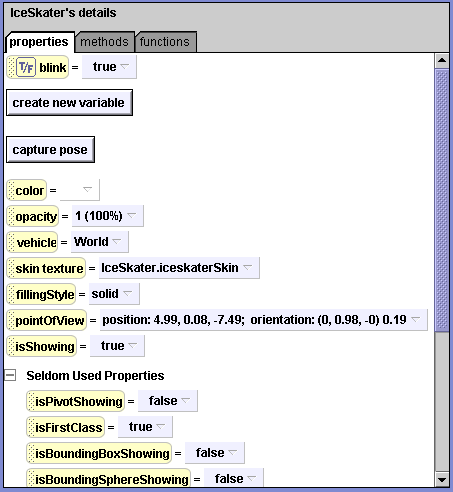
\includegraphics[scale=0.3]{Figures/aliceProp}} \quad
    \subfloat[Methods of an Object in Alice]{\label{fig:aliceComp-b}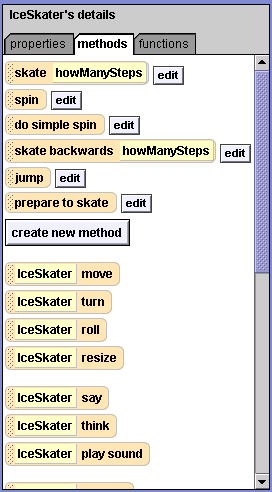
\includegraphics[scale=0.3]{Figures/aliceMeth}} \quad
    \subfloat[Functions of an Object in Alice]{\label{fig:aliceComp-c}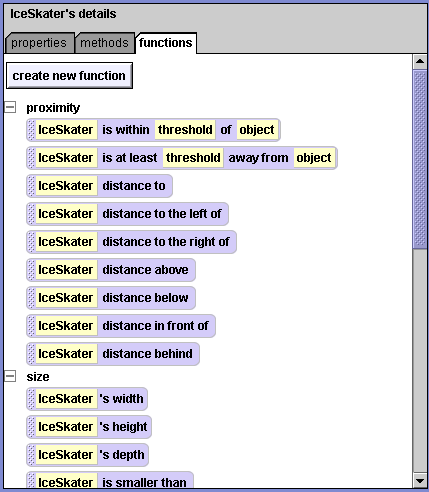
\includegraphics[scale=0.3]{Figures/aliceFunc}}
  \end{center}
  \caption{Components of the Alice Interface}
  \label{fig:aliceComp}
\end{figure}

Secondary notation can be related to visibility (see below), in that a secondary notation may be present, but if it is not readily apparent then its usefulness is somewhat diminished.  As well viscosity (see below) can impact secondary notation, as if a system is very viscous then changing the layout may be artificially difficult causing an aversion to changing the layout of a program after it has been initially constructed.  As well, if the structure is changed, then the secondary notation can go out of date and become a detriment to aiding understanding of a program.  Green also acknowledges that perhaps novices may benefit from a more constrained system in which secondary notation is minimized, but admits that this is pure conjecture and that more research needs to be done to confirm or deny this hypothesis \cite{green96}.

\subsubsection{Viscosity}
\label{viscosityoutline}

Viscosity measures resistance to change.  A system which is highly viscous is one where seemingly small changes require a relatively large amount of effort to undertake.  This can of course be dependent upon the specific change in question, but certainly some environments make changes more difficult than others.  Green identifies two particular types of viscosity:

\begin{itemize}
	\item Repetition viscosity, where one change implies that the same change will have to be made elsewhere a number of times
	\item Knock-on viscosity, where one change implies many other changes to the whole to restore consistency
\end{itemize}

An example of repetition viscosity would be changing the name of an identifier in a textual language as each use of the identifier will have to be changed to the new name.  An example of knock-on viscosity is changing the return type of a function, as this will require one to change all code which makes use of the return value of the function to make the program syntactically correct again.

Given how many software systems evolve over time viscosity is a rather important dimension.  Additionally from the perspective of students learning to program, oftentimes students will make mistakes early on and correct them after the fact.  If the system is highly viscous this can be problematic, as the effort to correct mistakes can become a deterring factor in a students motivation to produce a high quality solution rather than one that is ``good enough''.

Kelso notes that oftentimes VPE's suffer from viscosity problems due to the overhead of managing layout.  There is an overhead associated with laying out and rearranging components in a way that conveys extra meaning (aiding secondary notation), and without making the layout seem ``cluttered''.  He argues that this is an inherent problem in any VPE which requires manual layout and formation of links between components \cite{Kelso02}.  Additionally, an editor which enforces program correctness\footnote{Which many VPE's do given that one of the goals of a VPE is the removal of syntax errors} imposes an impediment on changing or rearranging components.

Viscosity can be related to premature commitment, as if one has to make a design decision too early it is probable that that choice will need to be revised.  If the system is highly viscous then those changes will be difficult to incorporate, whereas if it has low viscosity then the changes should be easy to implement.  That is, ideally a system which suffers from premature commitment should have low viscosity otherwise the problems related to premature commitment are amplified.

Given that the amount of time and effort to incorporate a change is dependent not only on the notation but also the specific change in question, viscosity has oftentimes been measured by implementing a small change to the rocket trajectory program\footnote{Described on page \pageref{rocketproblem}} to take account of air resistance, by exerting a drag proportional to the square of the velocity, and measuring the amount of time it takes to implement this change.

\subsubsection{Visibility}
\label{visibilityoutline}

Visibility concerns ``whether required material is accessible without cognitive work; whether it is or can readily be made visible, whether it can readily be accessed in order to make it visible, or whether it can readily be identified in order to be accessed'' \cite{green96}.  Related to visibility is juxtaposability, the ability to view two or more components side-by-side.


\subsection{Application of the Cognitive Dimensions Framework to Other Environments}

FIXME - recap findings in Green and Kelso, and compare with discussion of gem cutter.